\chapter{Requirements and Naive Designs}
Section \ref{sec:3compare} concluded that recent advancements in interconnect standards try to tightly couple attached devices to host processor cores at an order-of-magnitude larger bandwidths. This has serious implications for accelerator design and, more importantly, for feeding them.\\
This chapter compares common accelerator memory access patterns and tries to generalize across several streaming-like access patterns. This benefits the data feeding architecture, since it will be applicable to a wider range of accelerators. Thereafter the merge-sort database operator is used as a case study to show that naive traditional design methodologies at these bandwidths will not suffice.





\section{Accelerator Classification}
\label{sec:class}
As mentioned in Section \ref{sec:adopt}, FPGA accelerators are most commonly used for a specific class of workloads. Therefore the memory access patterns found in these workloads are limited. The following list shows the most commonly found memory access patterns of accelerators including an example application \cite{li-mem-access}.
\begin{itemize}
  \item{\textbf{Complex} accesses are considered to be more difficult than for example strided access, but still regular and known a priori. An example is a Hessian computation found in augmented reality. Image processing also uses similar access patterns.}
  \item{\textbf{Gather} accesses multiple pieces of data from non-contiguous locations in host memory. Each request consists of an absolute address and an amount of data to retrieve. This type of access often occurs for vector arithmetic.}
  \item{\textbf{Indirect array} accesses an array using a second array: $A[B[i]]$. The data for $B[i]$ is retrieved and the returned value is used to access array $A$. An example can be found in calculating a histogram in image processing.}
  \item{\textbf{Linked-list} reads an address that points to another address and so on. An example could be a network controller that handles header and payload data structures. The header contains information regarding the payload and is typically stored as a linked-list.}
  \item{\textbf{Streaming} accesses continuous chunks of data from host memory and stores it into a local buffer for processing. Examples include encryption and video processing.}
  \item{\textbf{Strided} accesses chunks of data with a fixed distance from the current address, called strides. Matrix multiplication is an example of a strided access since columns of the matrix have to be read where the stride is the row size.}
\end{itemize}

%\todo{- Add figure of different access patterns.\\
%- you could call the stream buffer an implicit DMA, since it moves data around but only in reading fashion and no explicit read commands are made. Just a start and end address in shared coherent main memory.\\
%- what kind of access do gpus or intel phi for example have/allow?\\
%- find more sources on accelerator access patterns\\
%- how is dma and our buffer connected? why did we not use a dma?\\
%}

Typically a DMA engine is used to direct memory access between the host memory, over the interconnect, and the local memory on the accelerator. A DMA enables compute to operate in parallel with memory transfers and provides data in large spatial-continuous blocks of memory to the accelerator. From this list, it becomes apparent that only streaming access directly benefits from a typical DMA transfer. The other access patterns do not, since they require either spatial-continuous data from multiple starting addresses or a single element from multiple starting addresses. For the first case, multiple DMA transfers have to be issued sequentially or a scatter-gather engine could be used, where a list of transfers is provided. The latter case requires buffering, since transferring data element-wise is inefficient over the interconnect due to under-utilization of the available data bus. The complex access for example, would even benefit from less than a cache line\footnotemark~granularity of data. For the complex access, element granularity is preferred, where an element is the data size of a single piece of meaningful data. In the image processing example, the data of a single pixel. Element granularity access is not supported by current frameworks such as the Streaming Framework or SNAP, discussed in Section \ref{sec:capi-1.0}.\\
However, a generalization across several streaming-like access patterns can be made. This renders the buffer architecture applicable to multiple access patterns and takes it out of the design process of an AFU designer. While the three database operators mention in Section \ref{sec:aim} are streaming based, a smaller granularity allows for more flexibility, especially with other access patterns in mind. Streaming access is the simplest pattern, because spatial-continuous data is read from a single starting address. A similar pattern is the strided access because in essence it consists of multiple stream accesses at the same time, where the starting addresses are at equidistant. A generalization of the strided access is the gather access, where also multiple non-spatial-continuous locations in memory are read. However, the starting addresses do not necessarily have to be equidistant. Finally, the complex but regular access is a generalization across all of the previous patterns. It could require element-sized data from multiple memory locations at the same time. A buffer architecture with element-wise access enables, for example, the Hessian matrix complex access case. Each pixel required for the computation is located in a separate stream buffer, after which the accelerator is able to access each stream at any point in time.\\

\footnotetext{The data size transferred between the last level cache and host memory.}

As mentioned in Chapter \ref{sec:intro}, other students are studying three different accelerators for database operators: decompress-filter, hash-join, and merge-sort. In essence, each accelerator requires streaming access, but in different ways. The decompress-filter operator decompresses incoming compressed Parquet files and applies a certain filter to it. This accelerator exhibits perfect streaming access behavior. The merge-sort operator merges multiple pre-sorted key-value pair streams from main memory and merges them into a single sorted output stream. In the case of the hash join, while hash table accesses are irregular, an efficient implementation of hash-join will hold the hash tables in local memory such that the accesses to host memory are predominantly streaming.

%\todo{
%- Have to make the following bullet clear somewhere. Why do you not use a DMA or SG instead?\\
%- assess memory access of the three operators. use following link from Jian\\
%I just read an interesting paper from FPGA'16 named 'A Study of Pointer-Chasing Performance on Shared-Memory Processor-FPGA Systems'. I guess this would be a part of hash-join's memory access pattern. I am not sure whether this is useful for you. For quickly have a view of this paper, it studies a linked list traversal behavior on the shared-memory heterogeneous computer systems (CPU+FPGA) including Xilinx Zynq, Intel QuickAssist QPI FPGA Platform, and Convey HC-2EX. It points out that memory latency is an important impact for pointer-based applications and shows the potentials of using this kind of FPGA-CPU shared-memory architecture.\\
%}





\section{Merge-Sort Accelerator Case Study}
%\todo{
%- Why is cache useful? Answer: fpga has small memory. partitioning your problem for fpga, you have to keep in mind this memory limitation. since small memory requirement, the problem gets cache friendly.\\
%- memory latency for cpu is much lower than for afu. however afu runs slower so more latency is not a problem.\\
%- concern Andrew Martin about a cache for streaming applications in general. Why not use ’a shit ton of’ buffering instead to cover the latency instead of using a cache? That is what he did when building a sorter on an FPGA. Peter’s response: we try to generalize the shit ton of buffering, so basically taking it out of the design process of the AFU designer. our cache is basically a big buffer.\\
%}
%\todo{
%- mention also HBM (8GB for VU37P) as an advancement which makes heterogenous computing more interesting for memory bound problems.\\
%- Peter: "Nice aspect of sort is that it plays at all different levels of the system." Why is that the case?!\\
%}

The merge-sort operator is an interesting database operator since it inherently uses multiple streams of key-value pair data from host memory. The complexity of the operator comes from the merging of multiple streams, where the next chosen stream to read is unpredictable. For databases, key-value pairs are a common data type. A key is a unique identifier with a size of 8 bytes for example. Most important for the key size is that it is large enough such that no collisions will occur. The value could be actual data or a pointer to the actual data. Since the value could be a pointer, 8 bytes are sufficient to hold a 64 bit address. Combining both the key and value size results in a 16 byte key-value pair, referred to from now on as an element, and is the smallest amount of meaningful data.\\
As mentioned in Section \ref{sec:cacheline}, the cache line size for the POWER architecture is 128 bytes. This means that each cache line holds eight of such elements. A reasonable, but extreme, use case for a merge-sort operator would be to assume a system with 1TB of host memory capacity. The latest generation of Xilinx FPGAs support up to \SI{8}{\giga\byte} of HBM (or RAM, but our goal in this thesis is to keep up with the OpenCAPI bandwidth rather than HBM bandwidth). In order to merge-sort all pre-sorted streams in one pass, a total of 128 streams are needed. Sustaining throughput is difficult when using a single stream. The inherent requirement of multiple streams makes it easier to fully utilize the interconnect bandwidth since requests can be made concurrently. For example, in the scenario where eight elements from different streams are requested, a typical cache line granularity interface has to fetch eight cache line granularity data blocks, select the requested element from each cache line, and buffer or discard the rest. By using read ports with element granularity, no data is wasted.



\subsection{Naive Buffer Design}
\label{sec:naive-design}
Usually a buffer is placed between the incoming data interface and the data consumer (accelerator) since the availability and consumption of data may happen at different rates. A buffer is also used to hide the latency of the interconnect by placing the data close to the consumer. Since the addresses of all cache lines are known \textit{a priori} for the streaming and the streaming-like patterns discussed before, the cache lines can be easily pre-fetched to keep the buffers filled without having to flush the buffers since no data is fetched speculatively.\\
In order for the accelerator to keep up with the OpenCAPI bandwidth, it has to consume 128 bytes (cache line size) per cycle. The interface provided by the TLX to the AFU designer consists of 64 byte data buses, operating at \SI{400}{\mega\hertz}, over which 64, 128 or 256 bytes of data are transferred (taking one, two or four cycles, respectively). Since a cache line is 128 bytes in the POWER architecture, transferring less than that seems wasteful. When 64 bytes of data are requested for example, the CAPP fetches the requested 128 byte cache line and invalidates one half and transmits the other.\\
OpenCAPI supplies 64 bytes per cycle at \SI{400}{\mega\hertz} while a realistic target frequency for an accelerator is \SI{200}{\mega\hertz}. To cover an interconnect latency of \SI{1}{\micro\second} per stream (see Section \ref{sec:buffer-depth} for a more detailed explanation), 200 cache lines, or 256 when rounded up to the nearest power of two, have to be buffered on the FPGA per stream. Due to the unpredictable access pattern of the merge-sort, each stream has to be able to be read, thus have its own buffer, in any given cycle. The total buffer size \textit{B} for such an architecture can be calculated as shown in Equation \ref{eq:bbb}.
\begin{equation}
  B = N \times C \times L \implies 128 \times 128 \times 256 = \SI{4}{\mega\byte}, \text{where}
  \label{eq:bbb}
\end{equation}
\begin{itemize}
  \item{\textit{N} is the number of streams,}
  \item{\textit{C} is the cache line size in bytes, and}
  \item{\textit{L} is the latency to be covered for OpenCAPI (rounded up to the nearest power of two).}
\end{itemize}

As shown in Section \ref{sec:fpga-characterization}, the Xilinx FPGA from the Kintex+ product line has a BRAM capacity of \SI{4}{\mega\byte} and a URAM capacity of \SI{4.2}{\mega\byte}. This means that all BRAM or URAM resources are consumed by this naive buffer architecture, leaving no resources for additional control, and more importantly, the actual AFU. Both \textit{N} and \textit{L} in this equation are subject to change and pose a trade-off. Either have fewer streams or buffer fewer cache lines per stream. Fewer streams may not be problematic, depending on the application. Buffering less per stream means that for a worst-case latency scenario, the AFU has to stall since there is no meaningful data present in the buffer. This might not be a problem if the access pattern of the respective AFU is evenly distributed across all available streams (as is the case for the decompress-filter). However, in the case of the merge-sort, the access pattern is unpredictable across streams. In order to maintain the OpenCAPI throughput and support the worst-case, the number of streams is reduced to 64. This configuration consumes roughly half of all the available BRAM resources instead of all of them.



\subsection{Crossing the Cache Line Boundary}
\label{sec:boundary}
As previously mentioned, each cache line consists of eight key-value pairs or elements. Due to the absence of a cache or buffer in OpenCAPI 3.0, multiple smaller than cache line data granularity read ports are desired and would make the buffer architecture also more general. A cache would be nice but is difficult to keep coherent in the current state of OpenCAPI 3.0. Relying on software is expensive and results in overhead and increased latency. Because streaming-like patterns are targeted, a buffer is sufficient. In the future, the buffer could be extended to a cache.\\
In order to accommodate element-wise read granularity, the buffer has to have eight read ports to consume a cache line size of data every cycle. Each read port has to be able to supply an element from any of the available streams. Due to the nature of streaming access, the next read from a stream is always the next element. In essence there are four particular access patterns, shown in \autoref{fig:3-afu-access}, that are interesting to explore, since the buffer architecture has to be able to handle those access patterns. In this figure, each numbered block represents an element in a cache line. The number represents the offset within the cache line and if the element is green, the element is being read in order to show the access pattern.
\begin{itemize}
  \item{\autoref{fig:3-afu-access-1} shows the entire current cache line being read for a single stream. In this case, a single stream and cache line are being read.}
  \item{\autoref{fig:3-afu-access-2} shows the current cache line being read for eight different streams, each reading the next element at the respective offset per stream. In this case, eight different cache lines and therefore eight different cache lines are being read.}
  \item{\autoref{fig:3-afu-access-3} shows the current and next cache line being read, crossing the cache line boundary. Crossing a boundary implies that at any given moment from any stream, two consecutive cache lines have to be read in the same cycle. In this case, a single stream from which two cache lines are being read.}
  \item{\autoref{fig:3-afu-access-4} shows the worst case scenario. If four boundaries are crossed in a single cycle, four different streams and eight different cache lines must be read concurrently.}
\end{itemize}

% https://tex.stackexchange.com/questions/196481/problem-on-subfigure-2x2
\begin{figure}[H]
  \centering
  \begin{subfigure}[b]{0.475\textwidth}
    \centering
    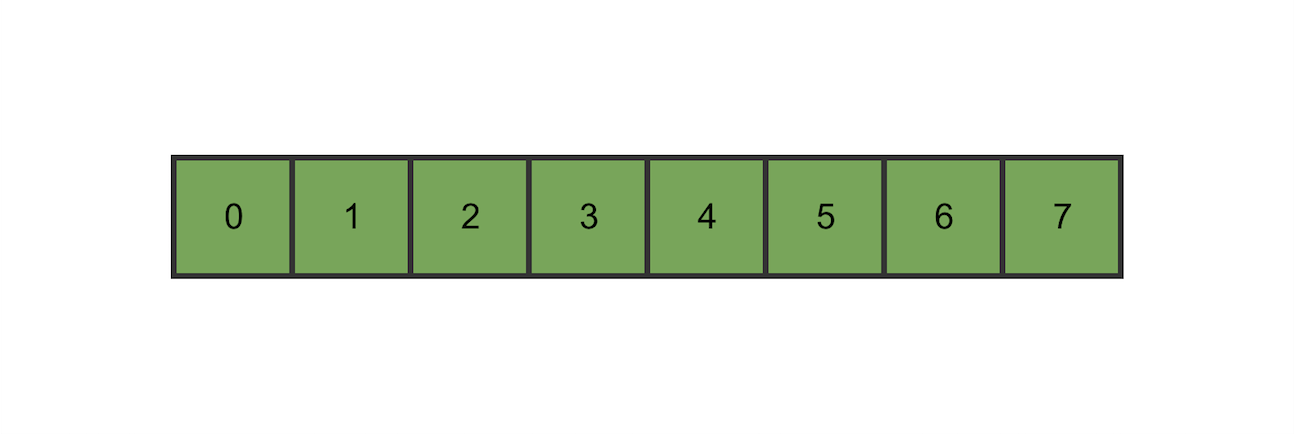
\includegraphics[width=\textwidth]{3-cross-boundary-1.png}
    \caption{Eight reads from a single stream.}
    \label{fig:3-afu-access-1}
  \end{subfigure}
  \hfill
  \begin{subfigure}[b]{0.475\textwidth}
    \centering
    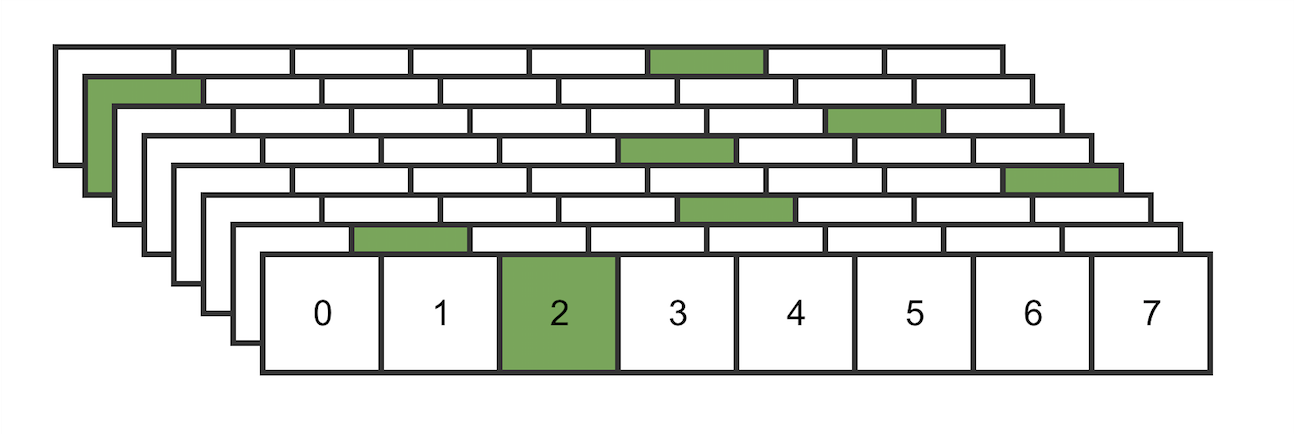
\includegraphics[width=\textwidth]{3-cross-boundary-2.png}
    \caption{Eight reads from eight different streams.}
    \label{fig:3-afu-access-2}
  \end{subfigure}
  \vskip\baselineskip
  \begin{subfigure}[b]{0.475\textwidth}
    \centering
    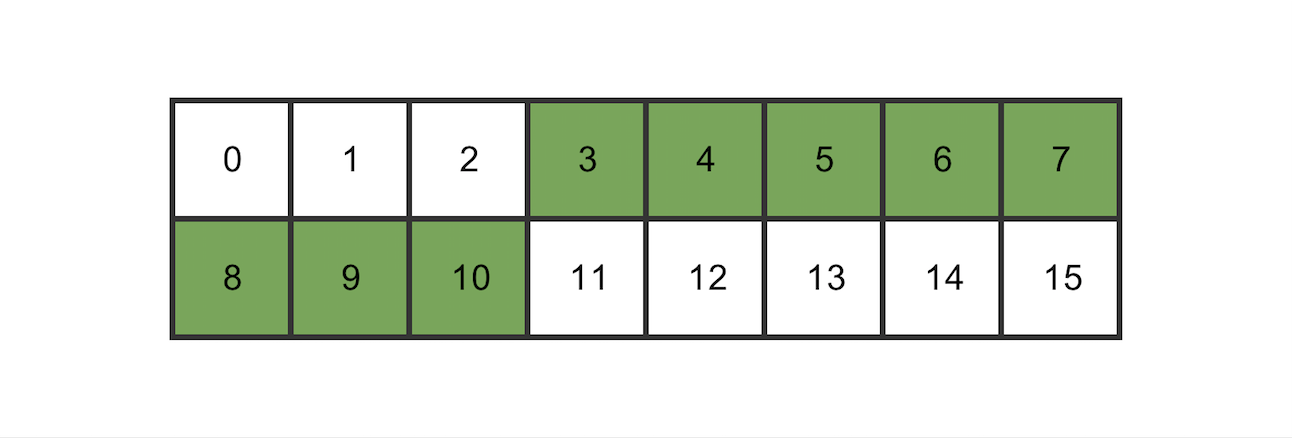
\includegraphics[width=\textwidth]{3-cross-boundary-3.png}
    \caption{Crossing a cache line boundary.}
    \label{fig:3-afu-access-3}
  \end{subfigure}
  \quad
  \begin{subfigure}[b]{0.475\textwidth}
    \centering
    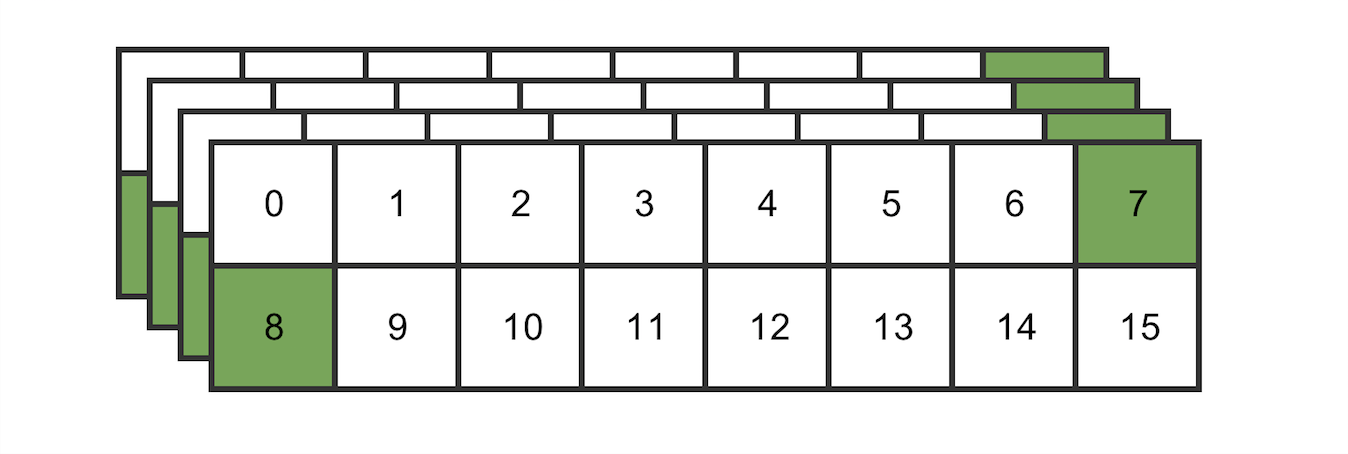
\includegraphics[width=\textwidth]{3-cross-boundary-4.png}
    \caption{Crossing four cache line boundaries.}
    \label{fig:3-afu-access-4}
  \end{subfigure}
  \caption{Four AFU access patterns using an eight read port buffer.}
  \label{fig:3-afu-access}
\end{figure}

Internally increasing the cache line size will not solve the problem of crossing cache line boundaries because the new boundary can also be crossed at some point. In essence, besides requiring a large memory to buffer the proper number of cache lines per stream, an eight read port memory is required with the granularity of a single element. This problem becomes less complex if the eight read ports would be constrained in a certain way. For example, by dividing the number of streams by the number of read ports and have each read port be dedicated to a subset of the streams. However, this contradicts the desire to keep up with the high-bandwidth and low latency interface provided by OpenCAPI. For unpredictable access patterns across streams, certain read ports may have nothing to do because of such a constraint. It also limits the access pattern generalization to not exclusively support purely streaming accesses.





\section{Design Requirements}
\label{sec:reqs}
It has become clear that a buffer architecture is needed for accelerators with streaming access patterns for which we wish to fully utilize the high-bandwidth and low latency interface of OpenCAPI. In order to do so, an access pattern generalization has been made that requires multiple read ports to concurrently and independently read from multiple independent streams of data. The merge-sort case study showed that a first-order naive design approach is not able to solve this problem and that care must be taken in order to maintain the design philosophy of high-bandwidth and low latency memory access for FPGA accelerators. Based on the previous chapters, the following is a set of requirements to which the final design has to comply in order to achieve these goals.

\begin{itemize}
  \item{Buffer 64 different streams in order to sustain the high bandwidth of OpenCAPI.}
  \item{Cover the OpenCAPI latency of \SI{1}{\micro\second} per stream.}
  \item{Go from 128 byte read port granularity to 16 byte data element granularity.}
  \item{Provide eight individual read ports such that if one read port cannot continue, the rest can still make progress.}
  \item{Handle reading across multiple cache line boundaries in a single cycle.}
  \item{Provide read ports with a low-latency between read request and data response.}
  \item{Provide a simple AFU interface by requesting data elements using stream identifiers. Streams are initially functionally reset such that an AFU has no knowledge of the addresses used.}
  \item{Provide a simple but generic interconnect interface that can be bridged to any current or future interconnect standard.}
  \item{Target the KU15P FPGA since the design can be scaled to fit the VU37P. Especially due to the vast increase in number of GTY transceivers, multiple OpenCAPI bricks can be attached.}
  \item{Confirm that the reference DLX and TLX design, provided by the OpenPOWER Foundation, also fits on the FPGA.}
  %\item{What kind of interface will I provide to the AFU designer? AXI (stream)?}
  %\item{Extendable in the future to a cache.}
\end{itemize}

%Work Element Descriptor (WED):\\
%- how will the WED look like, will there be a job queue or just a MMIO space on the AFU which holds the address in main memory of the job for each thread (context).\\
%- work element descriptor, what will it look like in a general case?\\
%- How does FU interact with memory? Does wed.source contain all information or is the AFU able to operate autonomously? Depends on application, some use WED work queue, others keep on sending WEDs instead.\\
%- support multiple engines in my framework. that means using and generating AFUTags (from the top of my head)\\





\section{Naive Design Exploration}
Section \ref{sec:naive-design} showed that a traditional approach of placing a buffer between the OpenCAPI interface and the accelerator for each stream will not fit on the target FPGA. The additional problem is the possibility of reading across a cache line boundary as shown in Section \ref{sec:boundary}. While the number of streams, the number of cache lines buffered per stream, or both can be reduced, the difficulty at hand is the required eight individual read ports with access to two consecutive cache lines in every stream buffer. This problem can be generalized as an eight read-port memory. Since FPGAs do not have the same level of flexibility as an ASIC has in terms of custom multi-ported memory cells, a solution has to be found regarding the available memory primitives. There are several traditional memory organizations that enable multi-port read access, built from smaller memory primitives.

\begin{itemize}
  \item{\textbf{Banked Memory} divides the total memory capacity into smaller memories called banks. Read requests are distributed across the banks. If multiple requests require access to the same bank, arbitration is required.}
  \item{\textbf{Duplication} replicates the memory contents in multiple memories and divides the read ports among them. Care has to be taken in order to keep the memories synchronized. Either by writing to all memories simultaneously or by keeping a live value table that keeps track of where valid data is located.}
  \item{\textbf{Multi-pumping} enables sharing of a common resource by running part of the logic at a multiple of the global frequency. For example, a memory primitive can be run at twice the frequency, effectively doubling the read ports or the data width.}
  %\item{\textbf{Rotating Buffer} provides a single buffer interface to all read ports where the oldest data gets rotated out, the other data shifts and new data gets rotated in.}
  \item{\textbf{Multi-port Primitives} provide multiple ports to the same memory. Since the target device is an FPGA, custom cells are not an option, but BRAMs can be configured as a true dual port primitive for example.}
\end{itemize}

%\todo{
%- make sure that for each BRAM limited example, also the 18kb example is mentioned, which is just a 36kb BRAM but with half the data width.\\
%- When calculating the estimated sizes of MUX structures and number of BRAMs, include the calculations as an appendix.\\
%}




\subsection{Cache Line Interleaving}
For each stream buffer, both cache line \textit{N} and \textit{N+1} could be read in the same cycle, as illustrated in \autoref{fig:3-afu-access-3}. This can be achieved by using a banked memory organization and interleaving even and odd cache lines, as shown in \autoref{fig:3-interleave-1}. Each bank consists of half of the total number of cache lines per stream and is built from multiple BRAM primitives as shown in \autoref{fig:3-interleave-2}. BRAMs are chosen because there is not enough distributed RAM available. URAMs have a fixed configuration of 4096 entries. This is too large for a single bank and the access latency of DRAM is too high. Each BRAM is configured as a 512 entry, \SI{8}{\byte} wide memory, of which sixteen are needed per bank. Basically each BRAM holds half of a \SI{16}{\byte} element, where the element offset is denoted by the numbers zero through seven and each half is denoted by suffix \textit{a} or \textit{b}. The green box shows how a single element is divided between two BRAM primitives and each half is located at address zero. The entire cache line is spread horizontally across BRAM primitives and can be accessed by reading at the same address in all sixteen BRAMs simultaneously. Doing this in both banks yields two successive \SI{128}{\byte} cache lines from which a single \SI{16}{\byte} element has to be selected by means of a \SI{256}{\byte}:\SI{16}{\byte} multiplexer for each read port. This architecture works under the assumption of a streaming access pattern because only successive elements are read. In a single cycle, only elements in two consecutive cache lines can be read. Therefore, each bank does not have to have eight physical read ports, but the requested element can be read by selection. While this architecture works in theory, there are two distinct drawbacks: multiplexer logic and BRAM primitive usage.

%\begin{figure}[H]
%  \centering
%  \begin{subfigure}[c]{.5\textwidth}
%    \centering
%    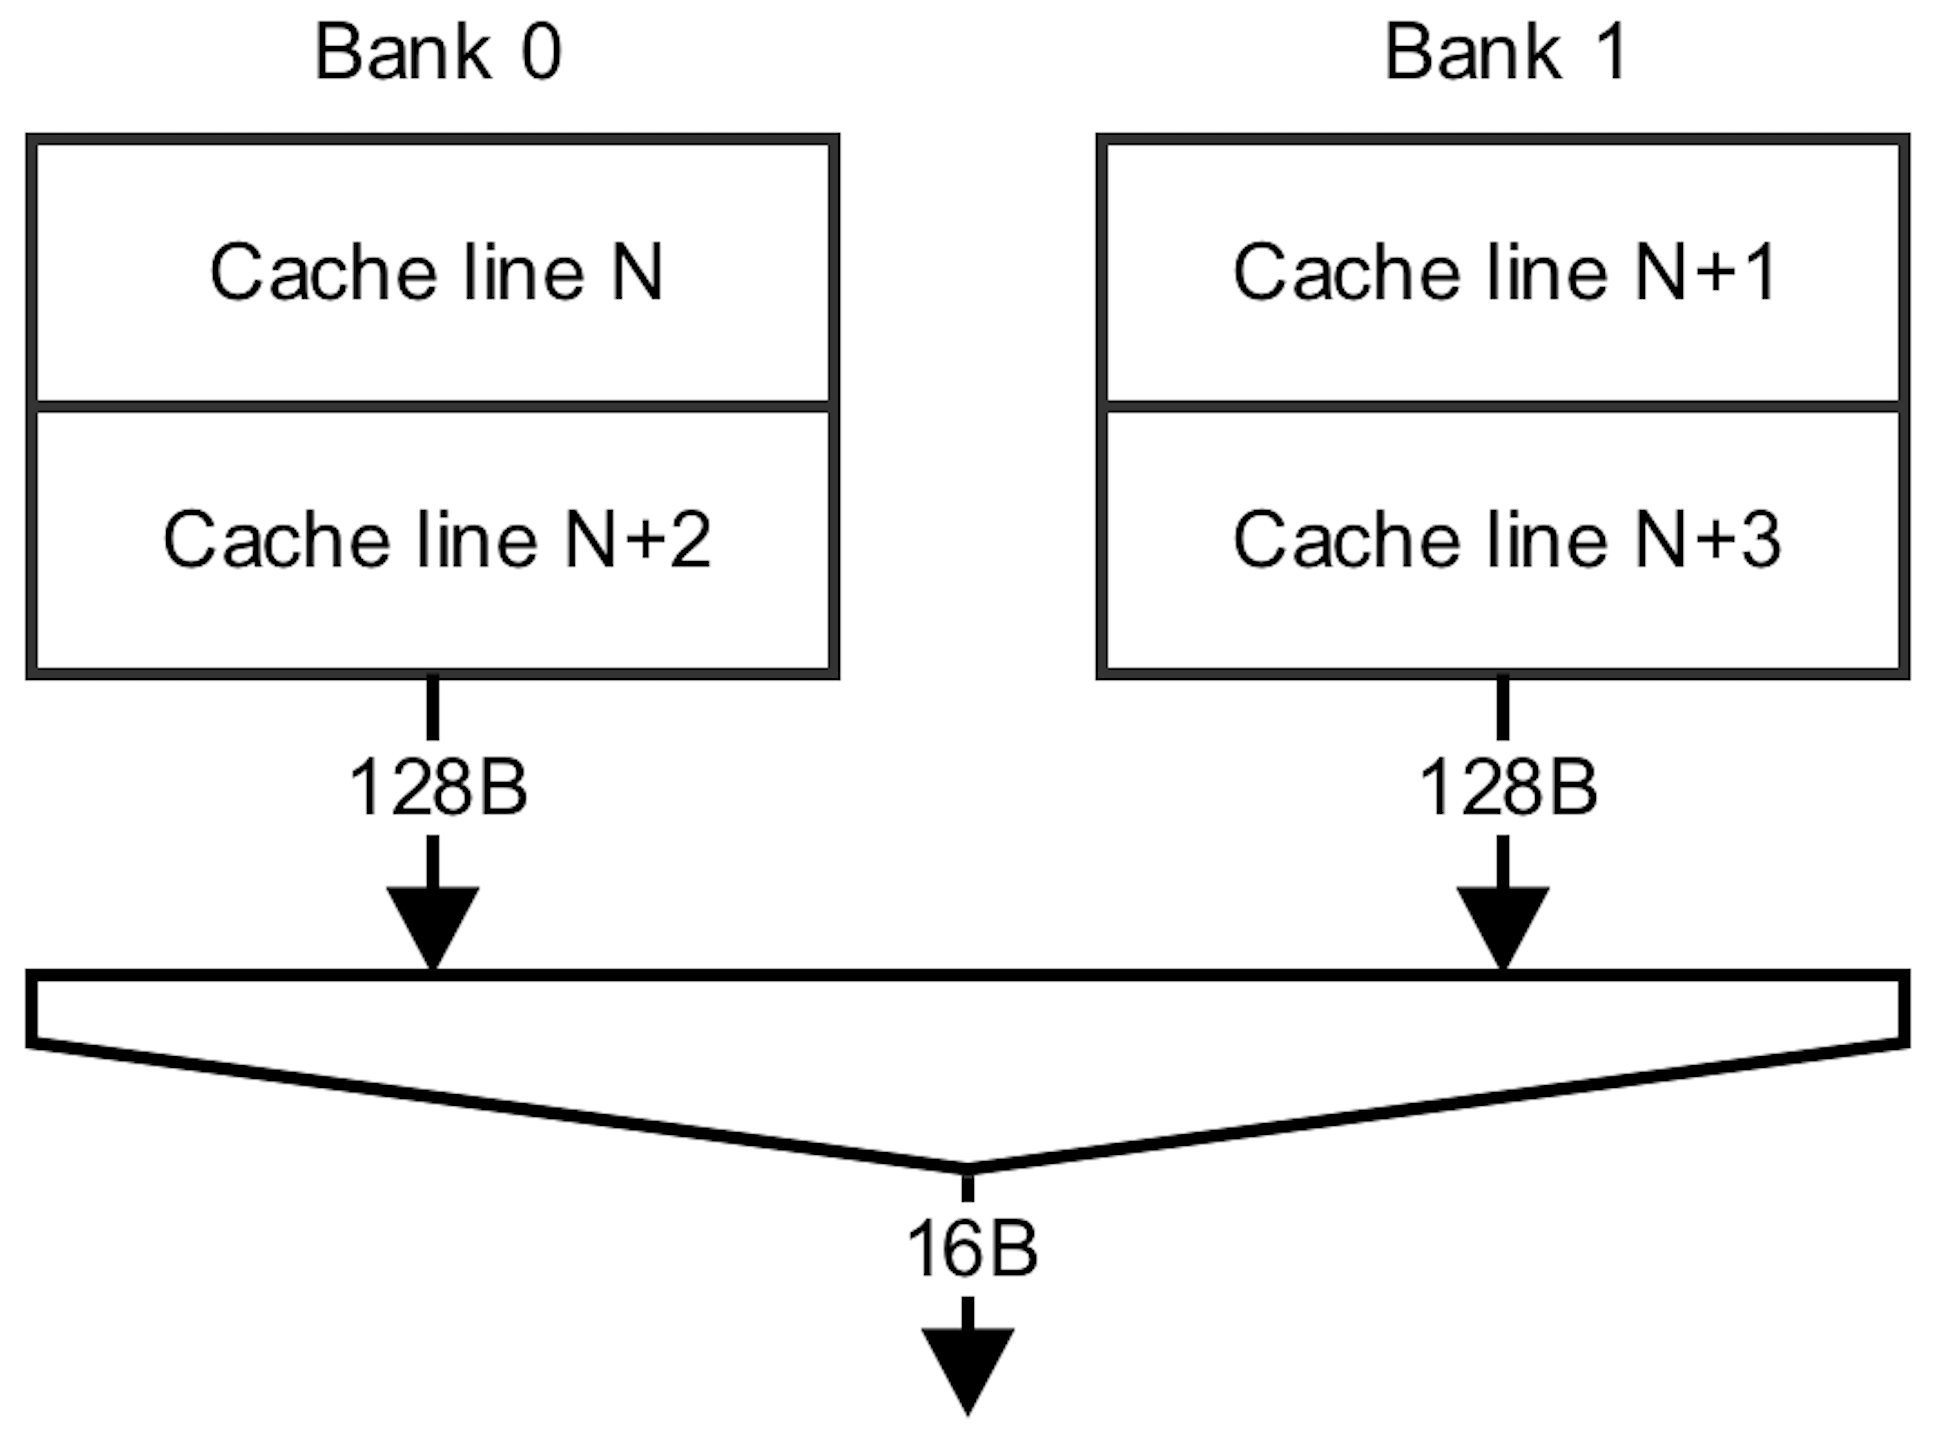
\includegraphics[width=0.7\linewidth]{3-interleave-1.png}
%    \caption{Two cache line banks per stream buffer.}
%    \label{fig:3-interleave-1}
%  \end{subfigure}%
%  \begin{subfigure}[c]{.5\textwidth}
%    \centering
%    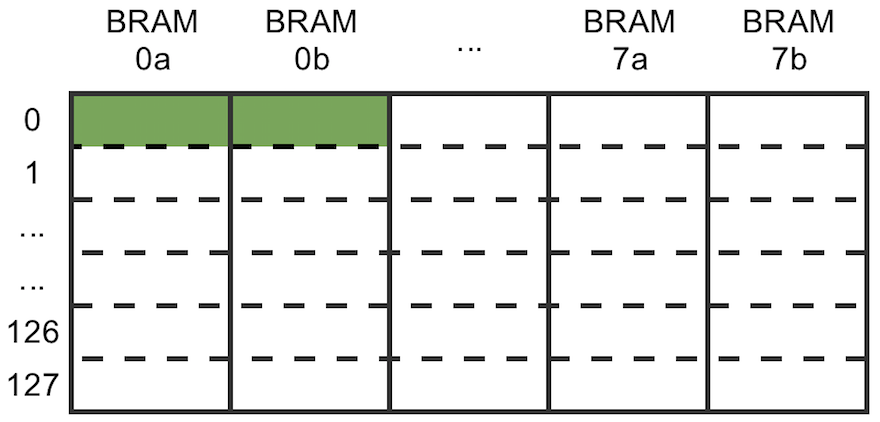
\includegraphics[width=0.8\linewidth]{3-interleave-2a.png}
%    \caption{Memory organization of a single bank.}
%    \label{fig:3-interleave-2}
%  \end{subfigure}
%  \caption{Interleaving even and odd cache lines.}
%  \label{fig:3-interleave}
%\end{figure}

\begin{figure}[htb!]
\ffigbox[\textwidth]
  {
    \begin{floatrow}
    \ffigbox[\linewidth]
      {\captionof{subfigure}{Two cache line banks per stream buffer.}
      \label{fig:3-interleave-1}}
      {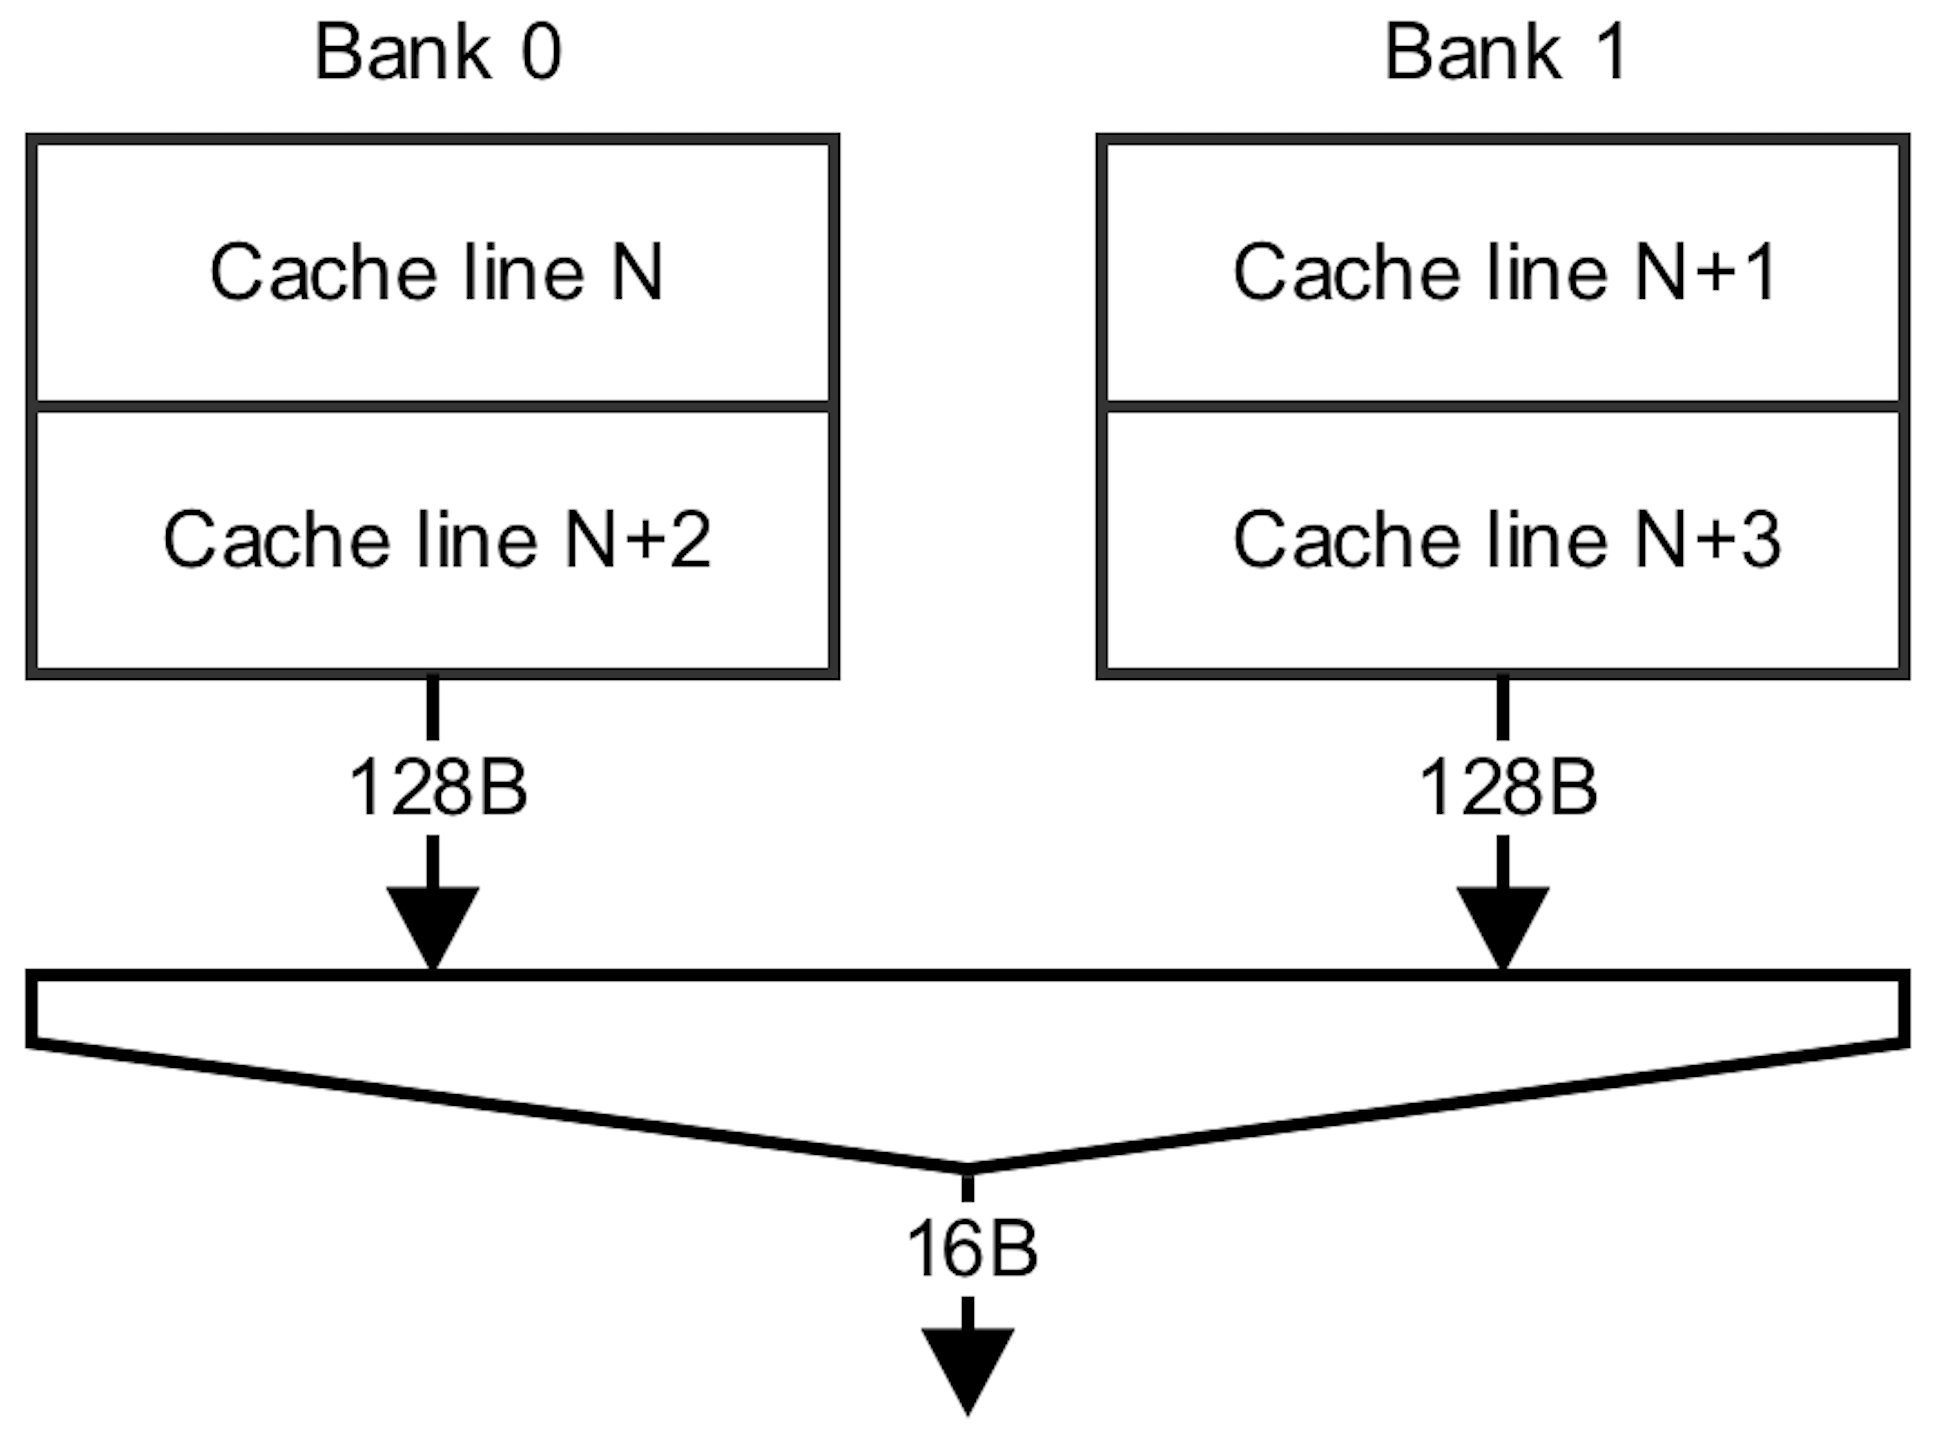
\includegraphics[width=0.80\linewidth]{3-interleave-1.png}}
    \ffigbox[\linewidth]
      {\captionof{subfigure}{Memory organization of a single bank.}
      \label{fig:3-interleave-2}}
      {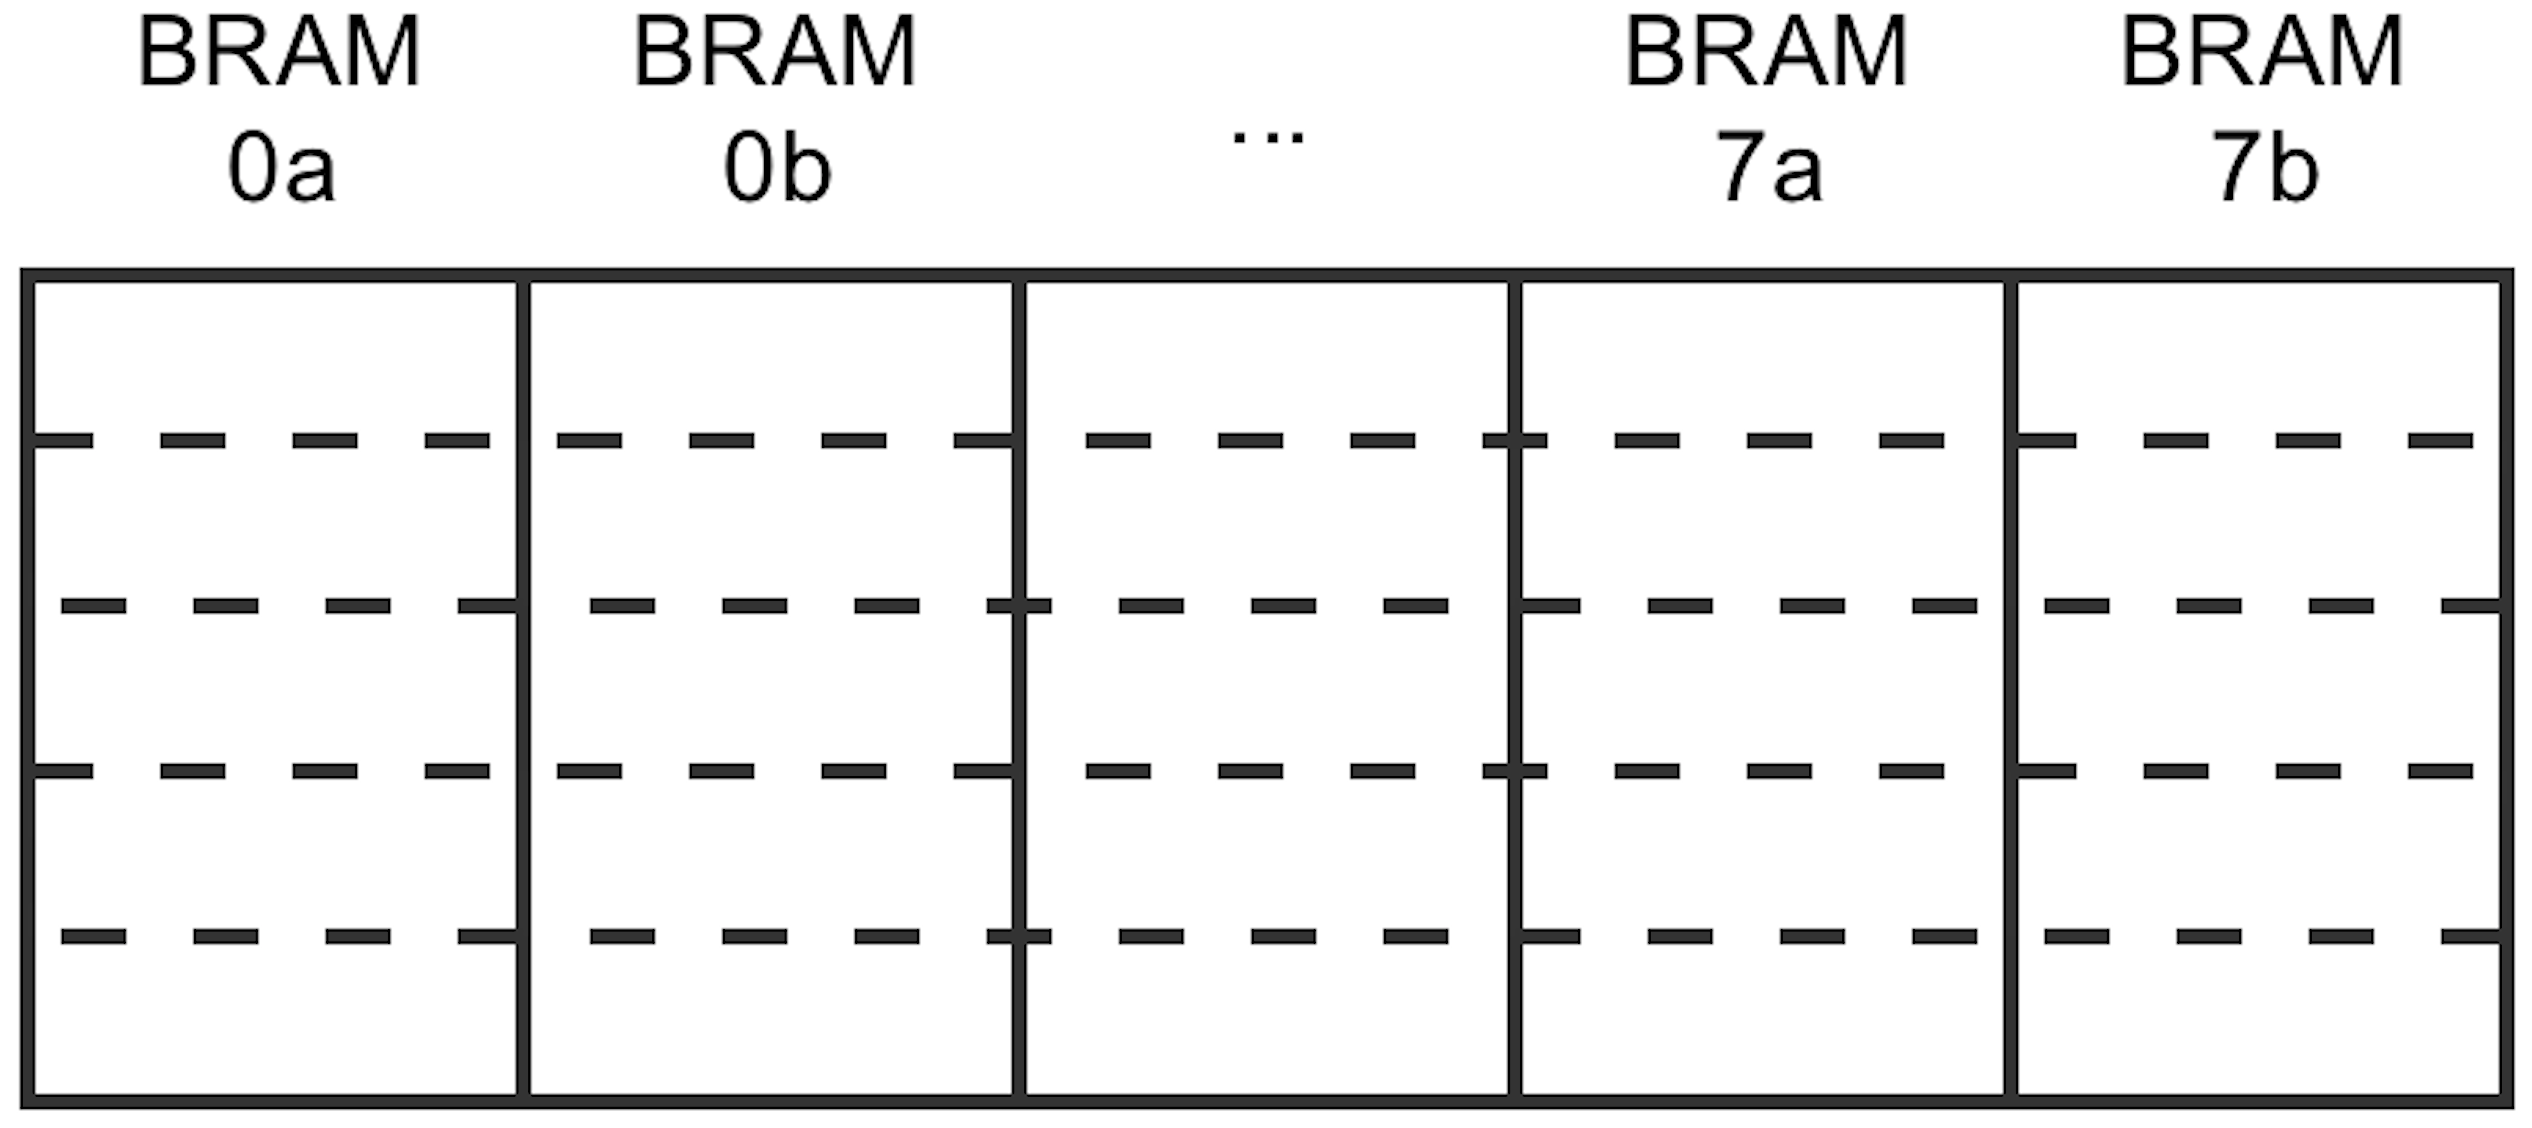
\includegraphics[width=0.80\linewidth]{3-interleave-2.png}}
    \end{floatrow}%
  }
  {\caption{Interleaving even and odd cache lines.}\label{fig:3-interleave}}
\end{figure}



\subsubsection{Multiplexer Logic}
In order to extract the correct \SI{16}{\byte} element from these two cache lines, the correct cache line (2:1 MUX) and the correct element (8:1 MUX) have to be selected. Since any read port can access any stream, the correct stream has to be selected, adding an additional 64:1 multiplexer. In total, each read port requires a 1024:1 multiplexer per bit of an element, resulting in 128 (16 bytes is 128 bits) of these multiplexers per read port.\\
Table \ref{tab:mux} summarizes several configurations of multiplexers after synthesis in the Xilinx Vivado 2017.1 tools targeting the KU15P. The column denoted by \textit{Ways} is the number of selectable inputs and \textit{Width} is the width in bits of each of those inputs. The estimation of the number of LUTs is based on the multiplex structures discussed in Section \ref{sec:clb}. Multiplexing of 32 or fewer inputs can be done within a single CLB. \autoref{fig:2-xilinx-mux} can be used to deduce the circuit for 16 or fewer inputs. For multiplexing 32 or more inputs, under the assumption that the number of ways is a power of two, the optimal structure of eight LUTs is multiplied by the number of times it is needed plus additional LUTs for selecting between the multiple optimal structures. An additional LUT is required for every multiple of four optimal structures, since a single LUT can act as a 4:1 multiplexer.

\begin{table}[H]
  \centering
  \caption{Summary of several multiplex configurations by estimation and after synthesis with the Xilinx Vivado tools targeting the KU15P.}
  \label{tab:mux}
  \begin{tabular}{ c | c || c | c }
    \multirow{2}{*}{\textbf{Ways}} & \multirow{2}{*}{\textbf{Width}} & \multicolumn{2}{c}{\textbf{LUTs}} \\ \cline{3-4}
                  &     & \textbf{Estimation} & \textbf{Vivado} \\ \hline \hline
    8             & 1   & 2                   & 3 \\
    8             & 64  & 128                 & 192 \\
    8             & 128 & 256                 & 384 \\
    16            & 1   & 4                   & 5 \\
    32            & 1   & 8                   & 9 \\
    64            & 1   & 17                  & 18 \\ % vivado guess
    128           & 1   & 33                  & 34 \\
    256           & 1   & 66                  & 68 \\
    512           & 1   & 132                 & 137 \\
    1024          & 1   & 264                 & 273 \\
  \end{tabular}
\end{table}

\autoref{tab:mux} shows that the synthesis tool always consumes more LUTs than expected. LUTs can also be used for routing of wires or for multiplexing instead of the hardwired multiplexers available. It is clear that if the number of ways increases, the estimated and observed number of LUTs start to differ more, or in other words, as the number of wires increases and therefore the routing complexity, more LUTs are used for wiring. The table also shows that when the width is increased, the amount of LUTs increases linearly with the initial observation for eight ways. From these results an improved estimation regarding the total number of LUTs required can be made.\\
Using the synthesis result for 1024 ways times the element width times eight read ports results in 279552 LUTs. This is roughly 53\% of the total LUT resources available on the KU15P. Besides, such deep multiplex structures are required to be pipelined in order to comply with the target frequency of \SI{200}{\mega\hertz}. Depending on the number of pipeline stages, an increasing number of flip-flop resources are required that also decrease the available resources for control logic and the accelerator itself. Besides that, there is also demultiplexing logic required for distributing the read requests among the stream buffers. The bottom line is that building these multiplex structures is very inefficient in terms of FPGA resource utilization.

% LUT calculation: you have 8 read ports and each read port has a MUX of 1024:1 with a width of 128 bits. That means: 273 (1024:1) * 128 (bits wide. table shows that when width increases, Vivado LUTs increase with the same factor) * 8 (read ports)

Multiplexers can also be implemented using DSP slices. A single DSP slice can be configured as a \SI{48}{\bit} wide 2:1 multiplexer \cite{xilinx-ug579}. Slices can also be cascaded due to the internal multiplexer that selects between the two slice inputs and one cascaded input from another slice. Therefore, to implement a 1024:1 multiplexer, 512 slices are needed. Since each slice has a width of \SI{48}{\bit}, three slices will cover the width of a \SI{16}{\byte} element. A single read port requires 1536 slices. Thus a total of 12288 slices are required, which is more than six times as many slices as available on the KU15P.

% NOTE: Visual example of wide bus multiplexing is given on page 64 in \url{https://www.xilinx.com/support/documentation/user_guides/ug193.pdf}.

%\todo{Optional:\\
%- According to this Xilinx Application Note: \url{https://www.xilinx.com/support/documentation/application_notes/xapp522-mux-design-techniques.pdf} The most efficient implementation of a MUX is an 8:1 MUX in a single slice, since it will use four LUTs and three 2:1 MUX primitives available in the slice. This is best for area versus number of inputs. However, if a higher frequency is required, a different implementation can be chosen, also present in the source, which is then a 12:1 MUX.\\
%- different ways to implement a MUX, in FPGA it is as a LUT, but for an ASIC its different. Andy thought about building a MUX with ORs and using enable signals from BRAMs instead. Do calculation if that is smaller than using LUTs.\\
%- During each cycle a single stream buffer potentially has eight meaningful outputs which have to be routed to any of the read ports. In essence, that is a crossbar with 512 inputs and 8 outputs, resulting in a wiring nightmare. In order to solve that, you can reorder the bits as in the patent, but does not take away that it will not fit. number of wires do not decrease, just their length and crossing of them. patent: APPARATUS FOR UNALIGNED CACHE READS AND METHODS THEREFOR
%}



\subsubsection{BRAM Primitive Usage}
Besides the difficulty of selecting the correct element, due to using two banks per stream, each bank consists of half the number of cache lines. As discussed in Section \ref{sec:fpga-characterization}, there is only a limited number of different BRAM configurations. The 512 entry by \SI{8}{\byte} wide configuration has the smallest number of entries. A single cache line can be distributed over sixteen BRAM primitives, but each primitive will effectively only utilize 128 out of the 512 entries or 25\%, as shown in \autoref{fig:3-interleave-2}. This solution would use 2048 BRAM primitives which is roughly 208\% of the available resources.\\
One optimization is to double pump the BRAMs such that each BRAM houses a single element, denoted by the number zero through seven in \autoref{fig:3-interleave-3}. The green box shows that a single element is located within the same BRAM primitive: half at address zero and the other half at address one. A cache line is horizontally spread over the eight BRAM primitives and vertically over two indices within a primitive. Double pumping results in utilizing 50\% of each BRAM and 104\% of the total BRAMs available.
% If each BRAM would be utilized fully, bank conflicts can arise because different streams are mapped into the same memory primitive. Additional logic is required to resolve such conflicts and will limit throughput or require clever scheduling.

\begin{figure}[H]
  \centering
  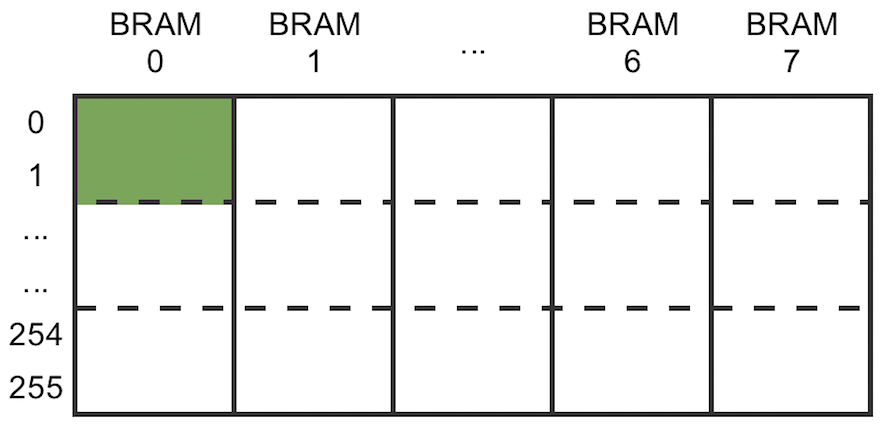
\includegraphics[width=0.40\textwidth]{3-interleave-3a.png}
  \caption{Memory organization of a single double-pumped bank.}
  \label{fig:3-interleave-3}
\end{figure}



\subsection{Element-wise Double-pumping}
\label{sec:wise}
By observing the streaming access pattern more closely with respect to the organization of BRAM primitives, it is clear that when a cache line boundary is crossed, each offset is read once per cycle at most, but never twice at the same offset. By exploiting this observation, a variation of the previous solution is possible which removes the need for two banks per stream buffer. \autoref{fig:3-element-wise-1} shows a single stream buffer where eight horizontal BRAMs contain a cache line. Each BRAM is double pumped as shown in \autoref{fig:3-element-wise-2}. The green box shows that a single element is located within the same BRAM primitive, similarly as in the previous solution.\\
Since two banks are no longer required, all cache lines fit within the same primitive resulting in a utilization of 100\% per BRAM primitive. For eight read ports roughly 52\% of the BRAM primitives are used. Also, there is no longer need for the first level of multiplexing, that reduces the per read port multiplexing to 512:1. Despite these improvements, this solution still requires 70144 LUTs utilize roughly 13\% of the resources.\\
While the design would fit theoretically, each BRAM primitive will have a fan-out equal to the number of read ports. Since getting data out of a BRAM and into processing logic is complex at the target frequency of \SI{200}{\mega\hertz}, the additional fan-out problem does not make this easier. Besides that, using more than half of the available BRAM primitives means that multiple large columns of BRAM primitives are used, scattered all over the FPGA as shown in Section \ref{sec:fpga-arch}. This complicates a unified access latency for each data entry (also keep the fan-out in mind) due to wiring delays across the entire FPGA. Pipelining helps with timing closure, but also increases the read latency of the buffer, a critical metric in the design.

% luts = 512 to 1 mux with 64b data width for 8 read ports. thus 137 * 64 * 8 = 70144 luts total. kut15p = 522720 luts. = 13.4\%\\

%\begin{figure}[H]
%  \centering
%  \begin{subfigure}[c]{.5\textwidth}
%    \centering
%    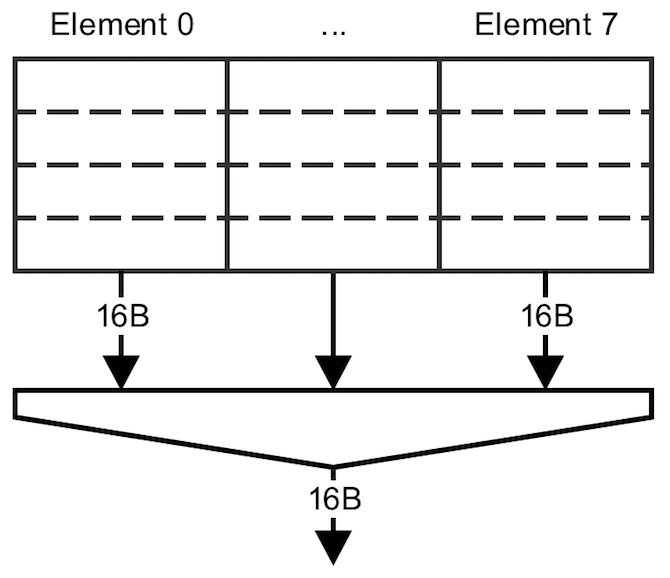
\includegraphics[width=0.6\linewidth]{3-element-wise-1.png}
%    \caption{Element selection from eight BRAM primitives.}
%    \label{fig:3-element-wise-1}
%  \end{subfigure}%
%  \begin{subfigure}[c]{.5\textwidth}
%    \centering
%    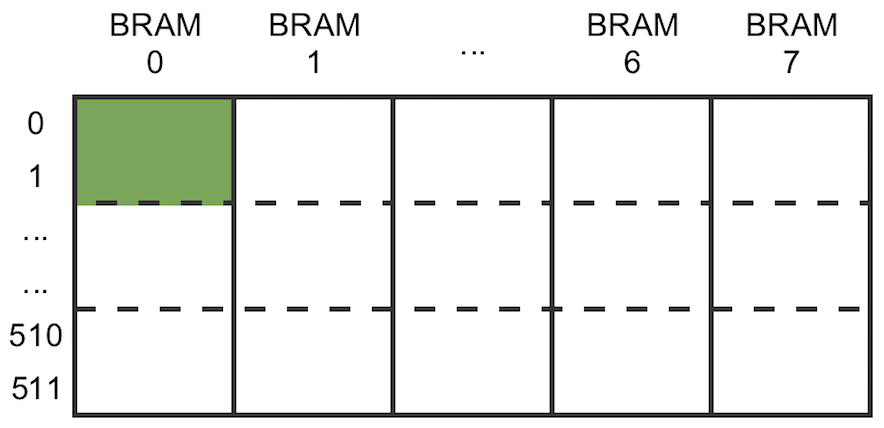
\includegraphics[width=0.8\linewidth]{3-element-wise-2.png}
%    \caption{Memory organization of a single stream buffer.}
%    \label{fig:3-element-wise-2}
%  \end{subfigure}
%  \caption{Element-wise double-pumping.}
%  \label{fig:3-element-wise}
%\end{figure}

\begin{figure}[htb!]
\ffigbox[\textwidth]
  {
    \begin{floatrow}
    \ffigbox[\linewidth]
      {\captionof{subfigure}{Element selection from eight BRAM primitives.}
      \label{fig:3-element-wise-1}}
      {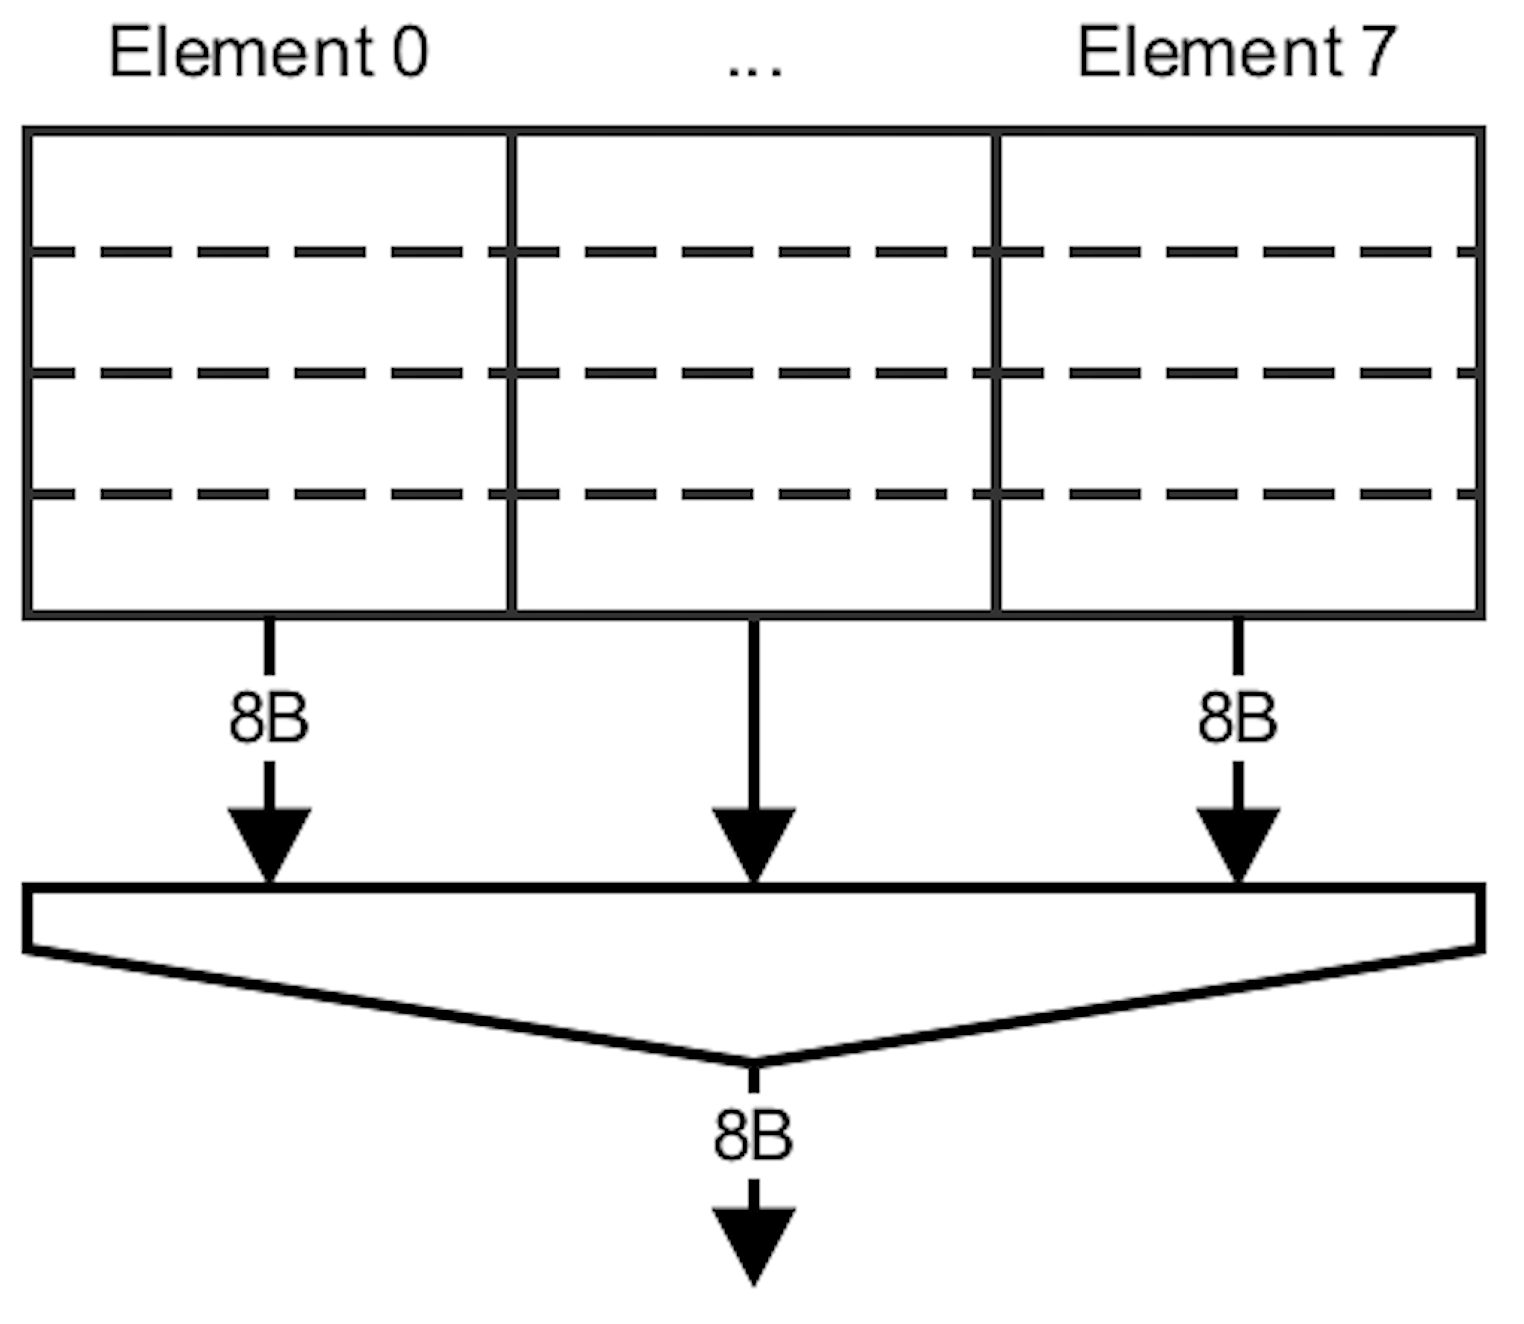
\includegraphics[width=0.65\linewidth]{3-element-wise-3.png}}
    \ffigbox[\linewidth]
      {\captionof{subfigure}{Memory organization of a single stream buffer.}
      \label{fig:3-element-wise-2}}
      {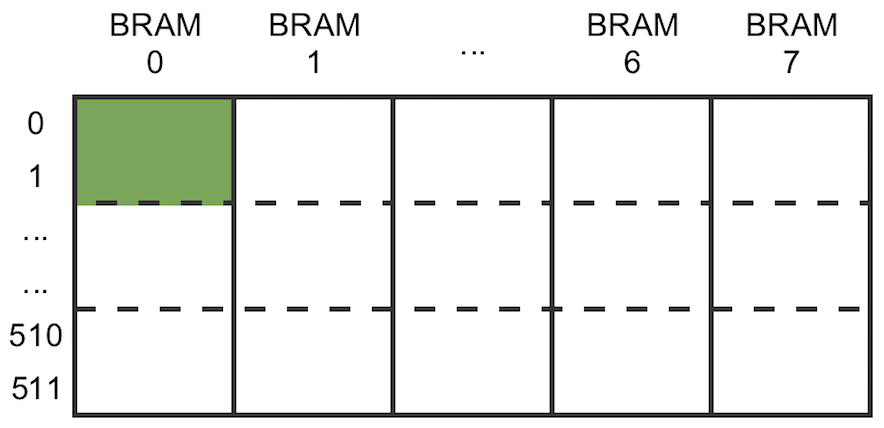
\includegraphics[width=0.80\linewidth]{3-element-wise-2.png}}
    \end{floatrow}%
  }
  {\caption{Element-wise double-pumping.}\label{fig:3-element-wise}}
\end{figure}



\subsection{Cache Line Duplication}
\label{sec:duplication}
Duplication guarantees that each read port has access to every element in every cache line at any time. \autoref{fig:3-duplication} shows a possible architecture for cache line duplication. Each read port has a copy of every cache line in each stream buffer, removing the need for large selection logic. The drawback is that the required memory primitives scale linearly with the number of read ports. As shown in Section \ref{sec:naive-design}, the number of supported streams has been decreased to 64 in order to save memory primitives and have resources to spare for control logic and the AFU. A single copy of all buffered cache lines for all streams requires roughly \SI{2}{\mega\byte} or 52\% of BRAM resources. This becomes \SI{16}{\mega\byte} or 416\% for eight read ports which is four times as much as available on the target FPGA. Each read port also has to select the right element. A 512:1 multiplexer is required and if the BRAMs are double-pumped, the total LUT consumption is roughly 13\%. It is obvious that this solution will not fit the target FPGA either. However, the benefit is that the wiring per read port stays within this slice that should make wire routing easier. Also the fan-out per BRAM output has decreased from eight to one, in comparison with the element-wise double-pumping proposal in Section \ref{sec:wise}.

%luts (best case with double pumping for mux reuse) = 137 (table) * 64 (data width) * 8 read ports

\begin{figure}[H]
  \centering
  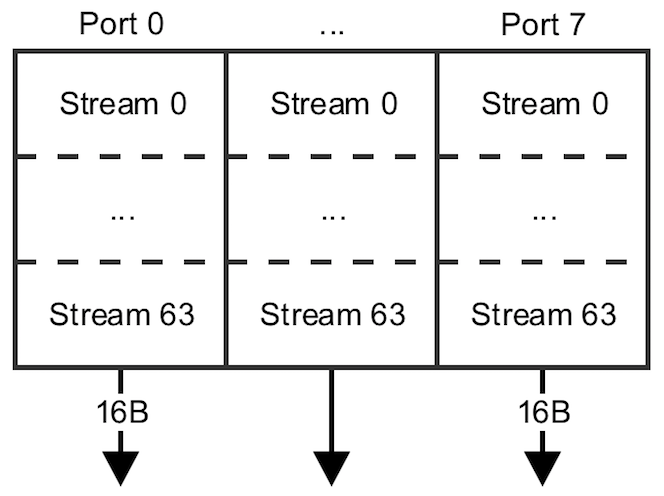
\includegraphics[width=0.30\textwidth]{3-duplication.png}
  \caption{Stream buffer duplication for each read port.}
  \label{fig:3-duplication}
\end{figure}



%\subsection{Rotating Cache Line Buffer}
%\todo{- add rotating buffer, see memory slides. similar to cell ask Peter how.\\
%- provides a buffer interface to each read port with two consecutive cache lines. When one is fully read, it will be shifted out and the next cache line will be placed in the buffer, therefore limiting the stream buffer to at most one read at cache line granularity per cycle.\\
%- specific to streaming access since you know you can keep part of the data since you will read consecutively.\\
%}

%\begin{figure}[H]
%  \centering
  %\includegraphics[width=0.90\textwidth]{1-model-of-computation.pdf}
%  \caption{.}
%  \label{fig:2-rotating-buffer}
%\end{figure}



\subsection{True Dual Port BRAM}
Finally, memory primitives can be used with multiple ports. A BRAM can be configured as either a simple dual port or a true dual port, as mentioned in Section \ref{sec:fpga-characterization}. In the case of a simple dual port, one port is a designated read port and the other a designated write port. The ports of a true dual port can be configured on-the-fly to act as either a read or write port. Due to the read-write imbalance of writing a cache line in one cycle and completely reading it for eight cycles, the flexibility of a TDP memory seems appealing. However, the effective capacity of a BRAM in TDP mode is reduced to \SI{18}{\kilo\bit}. Therefore, not only are twice the number of primitives required to obtain the same effective capacity, but also complex control logic to configure the ports on-the-fly is required. Even worse is that the previously used configuration of 512 entries is not available in TDP mode. Instead, the smallest number of entries is 1024 with a data width of \SI{36}{\bit}. This means that any of the previously discussed proposals will require twice as much BRAM primitives,not to speak about the additional control logic.
%Besides that, constraining concurrent reading and writing potentially limits throughput in specific cases. 



\subsection{Summary of Naive and Traditional Designs}
Traditional solutions for multi-ported memories have been shown above to not satisfy the desired requirements. Interleaving is an effective way to increase the number of read ports without increasing the required memory primitives. It does, however, pose the problem of under-utilized BRAM primitives and requires large multiplex structures that do not fit in the FPGA resource budget, not to speak of the wiring nightmare that will occur.\\
Element-wise double-pumping is a promising architecture. However, the fan-out of eight for every BRAM and the large columns of BRAM primitives scattered around the FPGA will require additional pipeline registers. This increases a critical metric: the read latency of the AFU.\\
While duplication solves the problem of the large multiplexing structures and the fan-out, there is no resource budget for it. Double-pumping BRAM primitives improves utilization and decreases the required LUTs, but does not solve the underlying problem.\\
The bottom line is that duplication is needed to mitigate the fan-out and, therefore, the wiring problem, but not for all cache lines.

%\todo{- mention rotating buffer; nice but limited to streaming. hurts throughput in more general case such as when changing this into a cache\\
%}



\section{Proposed Architecture}
\label{sec:final-design}
In essence there is a conflict between storing enough cache lines to hide the latency of OpenCAPI, and providing eight individual read ports to the AFU. Simultaneously, on the one hand wiring delay must be taken into account, and on the other hand not all of the available memory resources can be used. Therefore, the proposed multi-stream buffer architecture is split into two levels by exploiting different memory primitives. \autoref{fig:3-solution} shows both levels, \textit{L1} and \textit{L2}, analogous to cache naming conventions.
\begin{itemize}
  \item{\textbf{L1} is a 'small' buffer that is fed by L2. It stores a subset of consecutive cache lines per stream which are duplicated for each read port. This way, each read port has access to exactly the same data and there are no large multiplexer structures required.}
  \item{\textbf{L2} is a ‘big’ buffer that gets up to one new cache line every cycle through OpenCAPI. It is targeted to cover the latency of OpenCAPI by using large memory primitives and therefore does not consume all memory resources as was previously the case.}
\end{itemize}
L1 is optimized for low-latency and multiple read port access while L2 is optimized for memory capacity to cover the latency of OpenCAPI. By choosing the appropriate memory primitive for each level, an architecture can be devised that complies with the requirements and does not consume all available resources while doing so. To keep all duplicate cache lines synchronized in L1, L2 writes new data to all BRAMs simultaneously.

\begin{figure}[H]
  \centering
  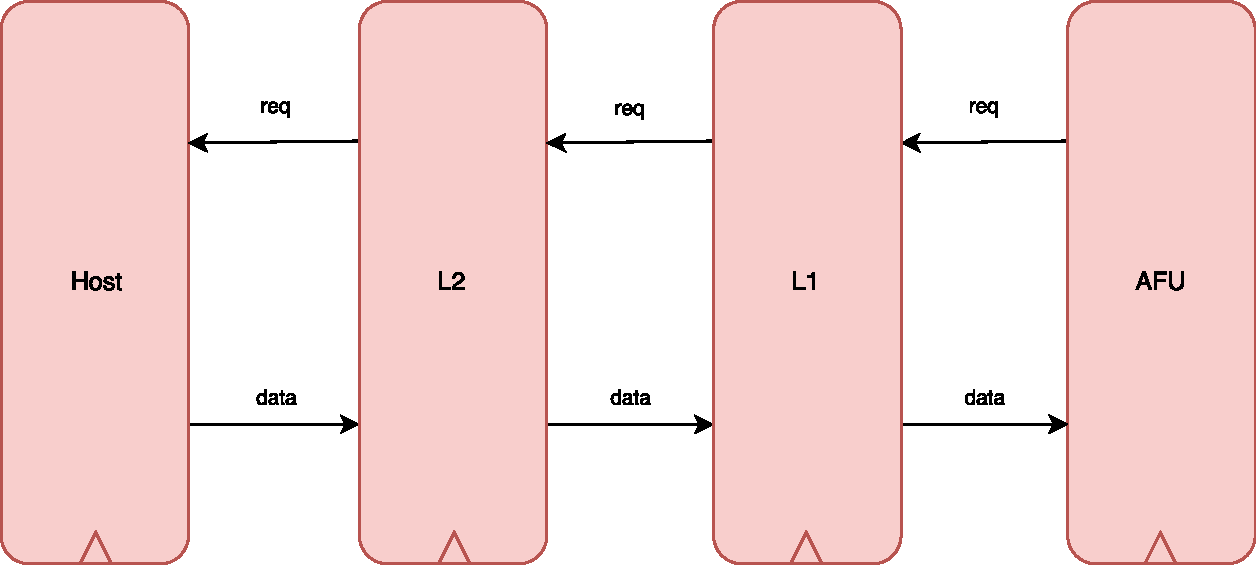
\includegraphics[width=0.70\textwidth]{3-solution.pdf}
  \caption{Proposed stream buffer architecture with two levels of buffering.}
  \label{fig:3-solution}
\end{figure}

The proposed architecture mitigates the fan-out problem from the critical AFU read path to a signal path outside of this domain, namely, between the L2 and L1 buffers. This gives us more time to move data out of the URAMs and into all BRAMs simultaneously. However, since cache line granularity data is moved from L2 to L1, the number of fan-out signals increases. Pipeline stages can be added to overcome this if necessary, due to the fact that memories are located in specific columns as shown in Section \ref{sec:fpga-arch}. The smaller BRAM arrays in this proposed architecture, as compared to the element-wise double-pumped architecture, make it easier to obtain unified access latency for each data entry. This is also achieved by supplying a BRAM array per read port such that cache lines used in the near future can be located closest to their consumer.\\
Since L1 is basically a smaller version of the proposed data duplication architecture, the same amount of LUT resources of roughly 13\% is required. Depending on the chosen configuration as to the number of streams and the number of cache lines, resource requirements differ. Section \ref{sec:design-choice} describes the design choices made in more detail.
